\Chapter{Megvalósítás}

\Section{A kód}
\SubSection{Kezdetek}
A legelején egy egyszerű python applikációba szerettem volna megvalósítani a megjelenítést és magát az egész projektet. Ehhez a TKInter nevű könyvtárat szándékoztam használni, állítható értékekkel, hogy megfigyeljem melyik érték kombinációval a legcélszerűbb a kép beolvasása és az adatok kinyerése onnan. Leegyszerűsített használatra, csak a sima akkordokkal foglalkozva ugye a kék színű akkordokat szándékoztam kinyerni a képből. Végül a csúszkákat félretéve manuálisan írtam át az értékeket, egy numpy (python függvénykönyvtár, többnyire tömbkezeléssel kapcsolatos) tömbbe csomagoltam be ezeket. Ezek az értékek kellettek ahhoz, hogy meghatározzam a cv2-nek, hogy milyen színskálába szeretném kiszedni az akkordokat. 
\par
Kísérleteztem azzal, hogy ha változtatom a skálát, akkor milyen pontossággal tudja visszaadni csak az akkordokat(amik kékkel vannak feltüntetve) a képről. Az volt a terv, hogy akkor ez mint bemeneti kép lesz majd kiolvasva a képből az OCR segítségével. Ehhez az kellett, hogy a megfelelő spektrumba legyen a program színhatára, amit ki tud olvasni zajmentesen, mivel a kották egységes kék színnel vannak kezelve akkordok terén, ezért nem kell egyáltalán változó értékű tömböket használni a színskála belövéséhez.
\par

\SubSection{A végleges program}
A következőkben áttértem jupyter-notebookra, hogy lehessen szétbontani, és emészthetőbbé varázsolni a kódot

\begin{python}
this_img = cv2.imdecode(numpyarray, cv2.IMREAD_UNCHANGED)	
\end{python}

\begin{figure}[h]
	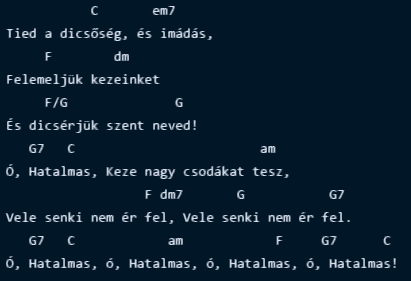
\includegraphics[scale=1]{images/output_tied.png}
	\caption{Az xml beolvasó program kimenete}
	\label{fig:output}
\end{figure}

Ez a fejezet mutatja be a megvalósítás lépéseit.
Itt lehet az esetlegesen előforduló technikai nehézségeket említeni.
Be lehet már mutatni a program elkészült részeit.

Meg lehet mutatni az elkészített programkód érdekesebb részeit.
(Az érdekesebb részek bemutatására kellene szorítkozni.
Többségében a szöveges leírásnak kellene benne lennie.
Abból lehet kiindulni, hogy a forráskód a dolgozathoz elérhető, azt nem kell magába a dolgozatba bemásolni, elegendő csak behivatkozni.)

A dolgozatban szereplő forráskódrészletekhez külön vannak programnyelvenként stílusok.
Python esetében például így néz ki egy formázott kódrészlet.
\begin{python}
import sys

if __name__ == '__main__':
    pass
\end{python}

A stílusfájlok a \texttt{styles} jegyzékben találhatók.
A stílusok között szerepel még C++, Java és Rust stílusfájl.
Ezek használatához a \texttt{dolgozat.tex} fájl elején \texttt{usepackage} paranccsal hozzá kell adni a stílust, majd a stílusfájl nevével megegyező környezetet lehet használni.
További példaként C++ forráskód esetében ez így szerepel.
\begin{cpp}
#include <iostream>

class Sample : public Object
{
    // An empty class definition
}
\end{cpp}
Stílusfájlokból elegendő csak annyit meghagyni, amennyire a dolgozatban szükség van.
Más, C szintaktikájú nyelvekhez (mint például a JavaScript és C\#) a Java vagy C++ stílusfájlok átszerkesztésére van szükség.
(Elegendő lehet csak a fájlnevet átírni, és a fájlban a környezet nevét.)

Nyers adatok, parancssori kimenetek megjelenítéséhez a \texttt{verbatim} környezetet lehet használni.
\begin{verbatim}
$ some commands with arguments
1 2 3 4 5
$ _
\end{verbatim}

A kutatás jellegű témáknál ez a fejezet gyakorlatilag kimaradhat.
Helyette inkább a fő vizsgálati módszerek, kutatási irányok kaphatnak külön-külön fejezeteket.
